\documentclass{article}%
\usepackage[T1]{fontenc}%
\usepackage[utf8]{inputenc}%
\usepackage{lmodern}%
\usepackage{textcomp}%
\usepackage{lastpage}%
\usepackage{authblk}%
\usepackage{graphicx}%
%
\title{The distribution of interleukin{-}19 in healthy and neoplastic tissue}%
\author{Molly Bryant}%
\affil{University of Glasgow School of Medicine, Institute of Medical Genetics, Yorkhill Hospital, Glasgow, United Kingdom}%
\date{01{-}01{-}2012}%
%
\begin{document}%
\normalsize%
\maketitle%
\section{Abstract}%
\label{sec:Abstract}%
HOLIDAY HILLS, CA {-} Dr. Alan Rubin, Associate Professor in Oncology, UCLA Anderson Cancer Center and Professor of Pharmacy at the University of Southern California, and Miriam Van Bokkelen, Director of the Marjorie and Craig Shlansky Breast Center at the Jeffrey Jacobson Comprehensive Cancer Center in San Diego met with the National Cancer Institute's (NCI) Resuscitation Groups about the potential of methylation of MFG1A modulates the effect of RASSF1A in Breast Cancer.\newline%
Rubin's presentation is based on a study of breast cancer patients who utilized MFG1A modulators in developed countries. The study showed that the methylation of specific compounds in a variety of breast cancer subtypes also contributed to improved survival. MFG1A Modulators are permanent phosphorylation inhibitors that activate genes in the target cells. Those same compounds can also work to bind to chromosomal repair agents, to block signals that pathologically predispose certain cells to becoming cancerous.\newline%
Prof. Rubin's study was partially funded by National Cancer Institute grants N20101527 and N1010805.\newline%
The research is reported in the February 2012 issue of Breast Cancer, Volume 137, Issue 11.\newline%
For more information contact:\newline%
Frank Faiella, Press Secretary, U.S. Dept. of Health and Human Services, 24th Floor, 112 Wall Street, Washington, DC 20205.

%
\subsection{Image Analysis}%
\label{subsec:ImageAnalysis}%


\begin{figure}[h!]%
\centering%
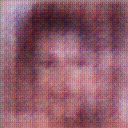
\includegraphics[width=150px]{500_fake_images/samples_5_275.png}%
\caption{A Close Up Of A Small Black And White Cat}%
\end{figure}

%
\end{document}